\documentclass[a4paper,12pt]{article}


%calling packages
\usepackage[english]{babel}
\usepackage[utf8]{inputenc}
\usepackage{amsmath}
\usepackage{graphicx}
\usepackage[left=1in,right=1in,top=1in,bottom=1in]{geometry}
\usepackage{setspace}
\usepackage[round]{natbib}
\usepackage{epstopdf}
\usepackage{soul}
\usepackage{lmodern}
\usepackage{caption}
\usepackage{hyperref}
\usepackage{subcaption}
\usepackage{rotating}


\usepackage{longtable}
\usepackage{amssymb}
\usepackage{fancyhdr}
\usepackage{array}
\usepackage{lscape} % for landscape formatting of pages
\newcolumntype{P}[1]{>{\centering\arraybackslash}p{#1}}
%fonts
\usepackage{times}
\setcounter{secnumdepth}{0}
%chanfing font of table headers
\captionsetup[figure]{labelfont=bf}
\captionsetup[table]{labelfont=bf}

%path to where figures are located
\graphicspath{ {images/} }

%for notes in table captions 
\newcommand\fnote[1]{\captionsetup{font=small}\caption*{#1}}

%changing header
\pagestyle{fancy}
\fancyhf{}
\rhead{\thepage}
\renewcommand{\headrulewidth}{0pt}
\renewcommand{\footrulewidth}{0pt}
\renewcommand*\footnoterule{}
\let\svfootnoterule\footnoterule
\renewcommand\footnoterule{\vspace{0.2in}\svfootnoterule}

%set spacing

\renewcommand{\sfdefault}{phv}

\doublespacing
\usepackage{titlesec}

\titleformat*{\section}{\Large\sffamily}
\titleformat*{\subsection}{\large\sffamily}
\titlespacing*\section{0pt}{24pt plus 4pt minus 2pt}{4pt plus 2pt minus 2pt}
\titlespacing*\subsection{0pt}{20pt plus 4pt minus 2pt}{4pt plus 2pt minus 2pt}


%changing title settings
\makeatletter
\renewcommand{\maketitle}{
	\begin{flushleft}
		
		\onehalfspacing
		
		\@title
		
		\lineskip .5em
		\normalfont{\normalsize{\@author}}
\end{flushleft}}
\makeatother


\newcommand{\beginsupplement}{%
	\setcounter{table}{0}
	\renewcommand{\thetable}{S.\arabic{table}}%
	\setcounter{figure}{0}
	\renewcommand{\thefigure}{S.\arabic{figure}}%
}


%title
\title{\bigskip \bigskip \sffamily \LARGE Responsiveness in Municipal Government}

%author
\author{\bigskip Benjamin Carl Egerod\footnote{Graduate Student, e-mail: \texttt{benjamin.carl.egerod@ifs.ku.dk}.} \qquad Martin Vinæs Larsen\footnote{Research Assistant, e-mail: \texttt{vinaes@gmail.com}.} \\ \textit{Department of Political Science, University of Copenhagen}} %e-mail



\begin{document}

	
	\begin{footnotesize} \noindent October 27 2017, Vejle. \end{footnotesize} %date
	
	\vspace{0.7in}
	
	\maketitle
	
	\bigskip
	
	\begin{quotation} %abstract

		\small \noindent \emph{Abstract:} Municipal governments supposedly empower citizens, giving them the ability to shape their local community based on their political beliefs. In spite of this, we know little about whether municipal governments are responsive to municipal electorates. In this study, we look at whether the policy implemented by local politicians actually respond to changes in the public mood. To do this, we compile a unique and comprehensive dataset of local fiscal policy, which we use to construct municipal-level estimates of fiscal policy conservatism. This detailed policy data is then linked to several measures of local ideological sentiment. We find strong evidence for dynamic responsiveness: if public opinion in a municipality changes, then public policy responds. We also look at whether single party control of the city council affects the level of responsiveness. We identify this effect using a close elections regression discontinuity design, comparing the responsiveness of city councils where the largest party narrowly won a majority of the seats with city councils where the largest party narrowly lost.
	\end{quotation}

\bigskip

\bigskip

\bigskip
	
	
	\noindent Prepared for the 49th Annual Meeting of the Danish Political Science Association \newline 
	
	\thispagestyle{empty} %removing page number from page one
	
	
	\bigskip
	\noindent \textit{Very early and incomplete draft.}
	\bigskip
	\bigskip
	
	
	
\section{Introduction}

In most developed countries municipal governments are an essential cog in the machinery of representative government. While they work within the framework of a national constitution and are generally subordinate to the central government, municipalities are, on average, responsible for a third of all public spending and, in most countries, they are able to levy taxes with little or no oversight \cite{oecd2016subnational}. In this way, they play a central part in the quintessential political act of deciding who gets what, when and how.  Yet until recently, we knew little about the extent to which municipal governments are actually responsive to their citizens preferences.


This changed with Tausanovitch and Warshaw's \citeyear{tausanovitch2014representation} recent influential study, which  was the first comprehensive examination of the responsiveness of city policy. In this study, \citeauthor{tausanovitch2014representation} used Multilevel Regression with Poststratification (MRP) to estimate the policy preferences of citizens in a cross section of all US cities with a population size of above 20,000, finding that there is a strong correlation between these preferences and city policy. Since the publication of this study, two other pieces of research has directly examined municipal responsiveness. The first of these are \cite{einstein2016pushing}. They also identify a strong correlation between citizen preferences, measured as support for the Democratic party at presidential elections,  and city policy in 2,000 midsize US cities. Other than replicating the findings from \citeauthor{tausanovitch2014representation}, \citeauthor{einstein2016pushing} are also able to identify the use of intergovernmental grants as a key mechanism underlying responsiveness (i.e., conservative cities are able to implement policies that differ from liberal cities because of these grants). They also offer a stronger identification strategy by identifying dynamic responsiveness \citep[cf.][]{stimson1995dynamic} in a panel of cities from two US states using a lagged dependent variable approach. In an unpublished study \cite{sances2017voters} expands on these findings using a panel of 3,000 US counties which spans the last 50 years. Linking changes in democratic vote share to county-level policy, \citeauthor{sances2017voters} finds that as counties grow more democratic they tend to spend more and collect more own-source revenues. This is even true within states, suggesting that the link between voter preferences and public policy are driven by local governments and not higher levels of government.

Aside from these studies, different strands of research has presented \textit{indirect} evidence that city policy might be responsive. For one, a number of recent studies have shown that voters tend to (re-)elect local politicians based on their actions in office \citep{arnold2012holding,burnett2017politics} and that voters tend to vote for conservative (liberal)  mayors if they themselves hold conservative (liberal) policy views  \citep{sances2017ideology,boudreau2015lost,hopkins2017retrospective}. Furthermore, a number of studies have found that it matters for city policy whether a conservative or liberal party controls the mayoralty and/or the city council \citep{fiva2016power,folke2014shades,blom2006parties,de2016mayoral}. 

%While these factors are necessary for the presence of municipal responsiveness, they are not sufficient. Even if voters tend to select politicians who share their ideological disposition, and even if these politicians tend to enact policies which reflect this disposition, these mechanisms need to operate in tandem, and be quite strong, in order to create responsiveness. If, for instance, politicians only have modest control over city policy, voters would need to send very strong policy signals through their vote in order for city policy to respond. 

All in all, research in the area of municipal reponsiveness has made impressive progress in the past few years, giving us evidence which strongly suggests that municipal governments are responsive to the concerns of their citizens. Even so, the existing evidence remains limited in different important ways.

For one, most of the existing studies, and \textit{all} the studies which study municipal responsiveness directly, focus exclusively on the US context. This puts into question whether voters are able constrain municipal policies in other contexts as well, or whether municipal responsiveness is a result of the particular features of the American political system. In relation to this, the existing studies all look at relatively large municipalities (\citealp{einstein2016pushing} has the smallest average municipal size of 40,000 inhabitants), making it unclear whether smaller municipalities, where politics is probably less professionalized, are responsive as well.

Furthermore, there seems to be a trade-off in the existing work between having good measures of city policy and voter preferences \citep[cf.]{tausanovitch2014representation} and having a stronger identification strategy \citep[cf.]{sances2017voters}. This is potentially problematic, as strong inferences about the extent of municipal responsiveness requires both high-quality measures and a convincing design.

Finally, existing work has primarily focused on identifying whether and when municipal responsiveness exists. As such, there is almost no causally persuasive work on whether certain municipal-level institutions can help promote (or depress) responsiveness.\footnote{\cite{tausanovitch2014representation} examines some interactions between different institutions and responsiveness, however, as they themselves recognize, these analyses suffer from substantial problems related to endogeneity.} 

In this study, we address these limitations related to context, design and data sources by studying responsiveness in Danish Municipalities. Danish municipalities are radically different from US counties and cities. They are small (average size 16,000), organized in general rather than special purpose governments \citep{berry2009imperfect}, lead by city councils which typically feature three or more parties, who are elected in a PR electoral system where turnout is relatively high. As such, if it is possible to identify responsiveness here as well as in the US, we can be pretty sure that municipal responsiveness is a relatively general phenomenon.

In order to identify responsiveness in this context, we develop an annual measure of municipal policy conservatives based on 14 fiscal policy indicators (1978-2006). A measure which is has much more comprehensive in terms of its granularity and the time period covered than the city policy measures used in previous studies. To measure the ideological sentiment in this time period, we use net support for conservative (right-wing) parties. Unlike previous studies, who have measured electoral sentiment using support for parties at national or regional elections, we are able to look at electoral support at \textit{local} elections dating back to 1970. (In a future iteration we will also use MRP estimates of citizen conservatism based on the Danish National Election Studies, however, we have not been able to do this yet.) These uniquely comprehensive data sources set makes it possible to  go beyond the trade-off between good measurement and a strong design which has characterized existing work. 



\section{Empirical Context: Danish Municipalities}	
Denmark is a decentralized welfare state where municipalities can affect their local revenue and set a yearly budget.  Municipal tasks and services include the core welfare services of the Danish welfare state and municipal spending amounts to 35 percent of GDP, which is more than half of all public spending.\footnote{The tasks include primary education, child care and care for elderly people, libraries, local sports facilities and other cultural activities, granting and payment of cash assistance, anticipatory pension and certain other social benefits, job activation and employment projects for unemployed persons (unemployment services), public utilities, environmental measures and emergency services.}


Danish municipalities are governed by small city councils (between 9 and 29 members) which are elected at proportional elections and with a multi-party system which, to a large extent, mirrors the party system at the national level \citep{blom2013et}. Elections are fixed to take place every four years and do not usually coincide with elections at the national or EU level.\footnote{There was only three years between the eelctions of 1981 and 1978} Turnout is high with an average of around 70 percent since 1970.  The work in the city council is structured by a a number of committees. The number and size of the committees is determined by the council. Committee membership is allocated proportionality between the political parties which means that there is broad political representation in all committees. The committees can decide on matters in their area and the administrative responsibility across areas is essentially divided. 

Following each municipal election, a majority in city council elects a mayor, and the chairmen of the various committees \citep{serritzlew2008explaining}. Mayors are the only full time professional politicians in the city councils and have a number of formal obligations \citep{kjaer2015urban}. Mayors are also responsible for the day-to-day business of the administration and chairs the important economic committee which sets taxes and the budget.


There have been two large municipal reforms in the last 50 years. The first was conducted in 1970 as the Danish welfare state started to expand. Here the number of municipalities were reduced from more than 1000 to 275.\footnote{In this study, we exclude the municipality of Copenhagen and Frederiksberg, as these were governed in a different way.} (Although it was 277 the first two years.) so that the municipalities were able to efficiently provide a more complex portfolio of public services \citep{ingvartsen1991kommunalreformen}. The second reform was conducted in 2007 and further reduced the number of municipalities from 275 to 98. Once again, the increasing complexity of public service provision was a key argument for the reform \citep{christiansen2008utaenkelige}. Since both of these reforms are so comprehensive, we let them be the bookends of our analysis, examining the relationship between citizens ideology and the ideological bent of city policy between the two reforms. Because of data availability we further censor the analysis to go between 1978 and 2008.

\section{An Annual Measure of Municipal Fiscal Policy Conservatism}
To measure fiscal policy conservatism in Danish municipalities we rely on 14 different indicators relating to either tax policy (3 indicators), spending policy (2), organization of public service delivery (3), co-payment for public services (4) or the extent of public services (2). While  spending and tax variables are commonly used in the literature, we are the first to include other types of variables in an analysis which is not simply cross-sectional. An overview of the policy indicators are presented in Table \ref{tab:policies}.

The included policies had to meet the following criteria: (1) The policy should be directly set by the city council.\footnote{Although it was included even if it was set in collaboration between the city council and some other  (set of) actor(s).} (2) It had to be a policy and not the outcome of a policy. (3) It had to be available for at least five years between 1978 and 2016. All policy information was retrieved from Statistics Denmark or the Danish Ministry for Economic Affairs and the Interior.

\begin{table}[h]
	\centering \footnotesize
	%\caption{Indicators of Fiscal Policy Conservatism}
	\label{tab:policies} 
	\begin{tabular}{p{5.5cm}P{3cm}P{4.5cm}} \hline
		\textbf{Policy}                          & \textbf{Availabiliy \newline (number of years)} & \textbf{Do Higher or Lower Values Imply Conservatism?} \\
		\hline
		&&\\ \textit{Tax policy} &&\\
		Income tax (pct.)                        & 29     &    Lower       \\
		Property tax (per mille)                      & 29    &    Lower        \\
		Commercial real estate tax (per mille) & 14    &    Lower               \\ \hline
	
		&&\\ \textit{Spending policy}  &&\\
		Spending pr. capita (DKK)                & 29    &    Lower        \\
		Spending pr. pupil in school (DKK)       & 7     &    Lower     \\ \hline
		
		&&\\\textit{Organization of public service delivery}  &&\\
 		Public Employees (pr. 1,000 citizens)	 & 9	  &	   Lower	     \\
 		Privately operated services  (pct.) &   14  &    Higher     \\
 		Purchases with a private supplier  (pct.)      & 14    &    Higher     \\ \hline
 	
 		&&\\ \textit{Co-payment for public services} &&\\   
		Average cost of day care (DKK)                  & 16    &    Higher     \\
		Price of relief stay (DKK)				 & 7	  &	   Higher	 \\
		Food delivery for the  elderly (DKK) & 7   &    Higher     \\
		Stay in nursing home (DKK)              & 7     &    Higher     \\ \hline
	
		&&\\ \textit{Extent of Public Services} &&\\ 
		Public housing (pct.)                    & 14     &    Lower               \\
		Class size in public schools	         & 14    &    Lower       \\
		\hline \hline
		\end{tabular}
\end{table} 

It should be noted that for most of our variables, data is only available after 1993, however, they still shape our estimates of municipal fiscal policy conservatism across the entire period, because of the Bayesian latent variable techniques, we make use of when creating the measure (more on this below).Even so, variables with missing values supply less information to the estimation in periods, where we have no data on them. Thus, estimates for the period 1978-1992 are based mostly on our measures of income and property tax as well as spending pr. capita.\footnote{To make sure that our results are not driven by the inclusion of different variables at various points in time, we have run all models using only those three variables, which does not change any results substantively.}

%\textbf{Maybe for later or the appendix coupled with analysis of beta-parameters etc.:} Furthermore, estimates of fiscal conservatism, when including all items and only the three with full coverage are highly correlated. It seems that the main difference bres is that the posterior distribution of the measure including all items exhibits lower variance. Additionally, the three items with full coverage have the most discriminating power, as shown by their higher $\beta$'s. This indicates that we are able to capture important aspects of fiscal conservatism with those three items alone. The addition of the remaining 11 variables serves to improve the estimation mainly by decreasing posterior variance.etween the two measu

\subsection*{Estimating Fiscal Policy Conservatism}
We conceptualize fiscal conservatism as a latent trait driving municipal expenditures, and rely on Bayesian latent variable modeling to estimate it. We parameterize fiscal conservatism through the following measurement model, which allows us to estimate it across time and space:

\begin{gather*}
F_{itk} \sim N(F^*_{itk}, \phi)\\
F^*_{itk} = \beta_k C_{it} - \alpha_{tk}
\end{gather*}

\noindent Where $F$ is the level of the observed fiscal policy variable $k$ in municipality $i$ at time $t$. the distribution of each of these observed variables is drawn from a normally distributed latent variable $F^*$, which has variance $\phi$. $C$ is the quantity of most interest -- the latent fiscal conservatism in that municipality. $\beta$ is the discrimination parameter, which captures how strongly each observed policy variable loads onto the latent dimension. Finally, $\alpha$ represents each item's difficulty parameter, which measures how fiscally conservative a municipality is, if it were to score 0 on the policy variable $k$. (Note that in future iterations, we will allow $\alpha$ to vary across time capturing that what was a highly conservative fiscal policy stance in 1978 is not necessarily as conservative in 2005.)

This parameterization is in many ways similar to frequentist factor analysis. However, a major advantage to using Bayesian techniques to make inferences about the latent trait is that the simulations will impute missing data during the estimation, which will allow us to include variables with different numbers of observations in the model -- the variables with missing observations will simply supply less information to the estimation. Furthermore, we can use the Bayesian priors to introduce dynamics into the model, thus allowing quantities to not only vary across time, but also directly model temporal autocorrelation. This is what allow policies which we have no information on in year $t$ to influence our estimate of policy conservatism in this year. Additionally, the estimation is simulation based, which allows us to directly estimate uncertainty around all model parameters. Finally, constraining prior distributions offers a flexible way of identifying the policy space. More on this final point later.

We include the 14 policy variables into the model. Before we do so, all variables are rescaled to have mean zero and variance one. Furthermore, all variables where higher values imply a more left-wing fiscal policy are reversed. This implies that when estimating policy conservatism, higher values on all variables indicate a more conservative policy.\footnote{This is strictly speaking not necessary, but it makes interpretation of the model parameters simpler.}

To identify the direction of the policy space, we constrain the $\beta$'s to be positive, so that municipalities scoring higher on our observed policy variables will be estimated to be more conservative. Location and scale is identified by placing standard normal priors on the distributions of all model parameters (hvad betyder dette?).

In our estimation, we run 7,500 iterations of the model, where the first 2,500 are burn in. We run three parallel chains. This gave posterior distributions with good properties (i.e., ?? ).

Figure \ref{fig:descriptive} presents some descriptive features of the annual measure of fiscal policy conservatism. In particular, it looks at how the measure is distributed across time and space, revealing some interesting patterns in municipal fiscal policy.


	
\begin{sidewaysfigure}[htbp]
\centering 
	\begin{subfigure}[h]{0.38\textwidth} 
	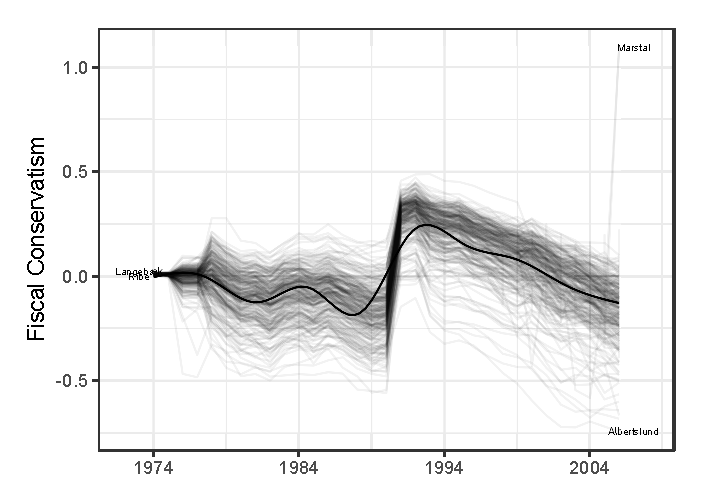
\includegraphics[width=1\textwidth]{times_lines_inflation_adjusted.eps}
	\caption{Average Municipal Fiscal Policy Conservatism (dark line) and Municipal Fiscal Policy Conservatism for Individual Municipalities (grey lines) from 1978 to 2006.}
	\label{fig:timeline}
			\end{subfigure} \hspace{1cm}
		\begin{subfigure}{0.38\textwidth} 
	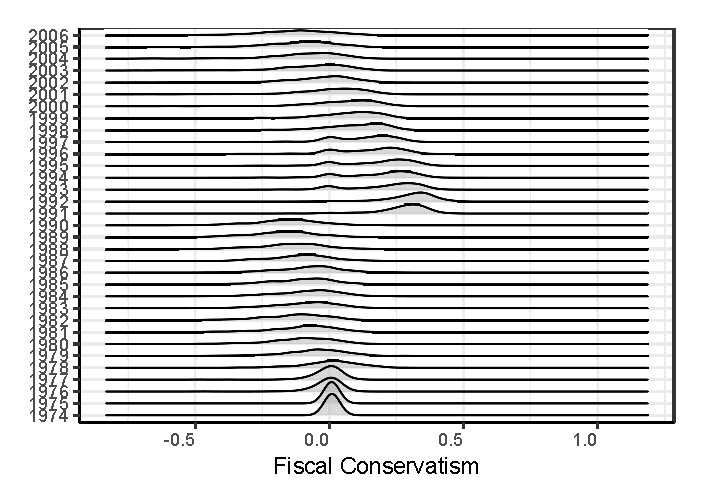
\includegraphics[width=1\textwidth]{JoyPlotFiscal_inflation_adjusted.eps}
	\caption{Distribution of Municipal Fiscal Policy Conservatism from 1978 to 2006 (densities).}
	\label{fig:lines}
	\end{subfigure}
		\begin{subfigure}{0.9\textwidth} 
	\includegraphics[width=1\textwidth]{Map_of_FiscCon.eps}
	\caption{The Geographic Distribution of Municipal Fiscal Policy Conservatism at Three Points in Time.}
	\label{fig:map}
		\end{subfigure} 
	
	\caption{How has Municipal Fiscal Policy Conservatism Developed from 1978 to 2006?}
	\label{fig:descriptive}
	
\end{sidewaysfigure}

\section{Measuring Local Policy Preferences}

In order to find out whether municipal fiscal policy conservatism responds to the preferences of the electorate, we need to develop a measure of whether voters in a given municipality prefers more fiscal conservatism or more fiscal liberalism. In line with previous work on municipal responsiveness \cite[e.g.,]{sances2017ideology,einstein2016pushing}, we measure local policy preferences indirectly by examining the net difference in electoral support for right-wing and left-wing parties in the municipality, inferring that municipal electorates who prefer conservative parties also prefer conservative fiscal policies. In particular, we looked at the difference between support for Venstre, Det Konservative Folkeparti, Fremskridstpartiet and Dansk Folkeparti (the major center-right parties as well as the right wing populist parties) and Socialdemokratiet, Radikale Venstre, Socialistisk Folkeparti, Venstresocialisterne, and Enhedslisten (the major center-left parties as well as the socialist parties) at all municipal elections in the period under study. This gives us an estimate of local policy preferences in the years 1974, 1978, 1981, 1985, 1989, 1993, 1997 and 2001. 

How well does this measure capture the municipal electorates underlying preferences? To get some indication of this, we look at the 2013 Danish Municipal Election Survey \cite{elklit2017kv13} where more than thirty respondents (avg. 46) from each municipality was asked to place them self on an eleven point ideology scale going from left to right. Using this data, we calculate the municipal specific mean of these responses and correlate this with the net support for conservative parties in the 2013 municipal election.  As can be seen from figure \ref{validation1} the two are moderately correlated, which suggests that we are in fact tapping into variation in policy views when we measure at citizens preferences over parties. The reader should note that the correlation is biased downwards, because we have random measurement error in our sample based measure. The reader should also note that due to the municipal reform of 2006 (cf. the section on empirical context) we can only have 98 observations corresponding to the 98 (amalgamated) municipalities.

\begin{figure}
	\begin{subfigure}{0.45\textwidth}
	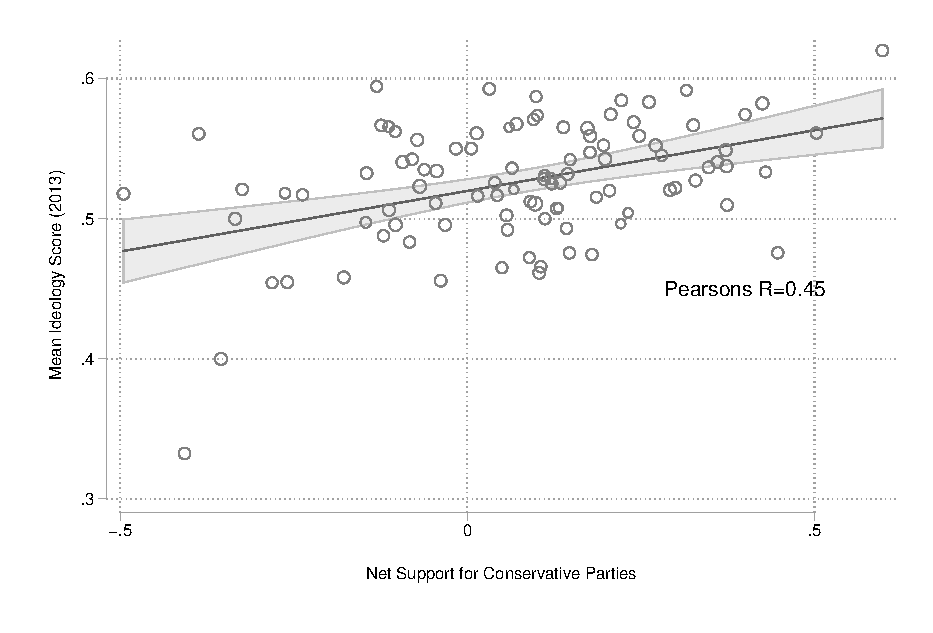
\includegraphics[width=1\textwidth]{validation.eps}
	\caption{Does the electorates preference over parties reflect preferences over policy? Data from the 2013 municipal election.} \label{validation1}
	\end{subfigure}  \hfill
	\begin{subfigure}{0.45\textwidth}
	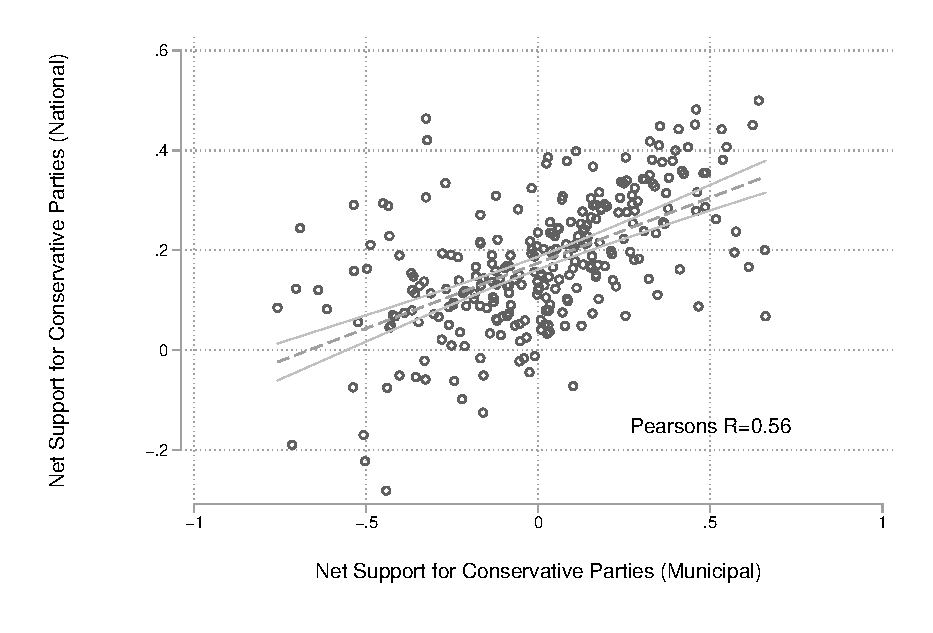
\includegraphics[width=1\textwidth]{validation2.eps}
	\caption{How strongly correlated are the electorates preferences at municipal and national elections? Data from the 2005 municipal and national elections.} \label{validation2}
\end{subfigure}
\caption{How does our measure of local policy preferences perform?}
\end{figure}

It is important to note that our measure of local policy preferences do not simply reflect the overall ideological mood in the municipality, but the ideological mood expressed by the electorate at municipal elections. This is potentially significant, because unlike previous research -- which uses national or regional electoral support --  we do not risk misidentifying electorates who might differ in their policy views across domains (i.e., who want more liberal fiscal policies locally and more conservative policies nationally). Why might there be such a divergence? For one, the electorate at municipal elections might be differently composed than electorates in national elections as different types of people participate in different types of elections \citep{ansolabehere2015beyond,hansen2017social} In addition to this, voters might have a preference over what level of government should be smaller and thus more fiscally conservative.

In figure \ref{validation2}, we try to gauge the extent to which our indicator of the municipal electorates preferences is improved by looking at municipal rather than national elections. In particular, we correlate  municipal-level  net support for conservative parties at the 2005 municipal elections with municipal-level net support for the same conservative parties at a national election held six months before. This analysis reveals a modest correlation of 0.56. Accordingly, there seems to be meaningful variation in local policy preferences that one does not adequately capture if one tries to use election returns from national elections.

How do our measure of local policy preferences relate to our measure of municipal fiscal policy conservatism? 

\section{Estimating the Level of Municipal Responsiveness}

We estimate the level of municipal responsiveness using the following model

\begin{equation}
 C_{it+1} =  \beta  V_{it} + \gamma_i +  \pi_t + \theta POP_{it}  + \epsilon_{it}
\end{equation}

Where $C_{it+1}$ is the change in municipal fiscal policy at time $t+1$ in municipality $i$, $V_{it}$ is the change in support for right wing parties at time $t$, $\gamma_i$ and $pi_t$ represent municipality and time fixed effects, $POP_{it}$ is the logged population size and $\epsilon_{it}$ is an error term.

The estimate of interest in this model is $\beta$ which signifies the marginal effect of the electorates preferences on municipal policy.

This model can be interpreted as a generalized difference-in-difference model, which looks at whether policy becomes more conservative in municipalities where voters become more conservative. Furthermore, there is a dynamic aspect to our analysis, in that we expect that the electorate preferences do not have an instantaneous impact. Rather, we expect that changes in voters preferences at time $t$ will affect policy at $t=1$. In particular, we look at effects four years down the line, as this corresponds to the election period in Danish municipalities. 

One advantage of using such a difference-in-difference model is that the identifying assumption (i.e., parallel trends) can be tested. In particular, we can see whether areas where voter preferences became more conservative had a different trend in policy conservatism than areas where voter preferences became less conservative.  


\subsection{Results}

Tor


\begin{figure}[h]
	\centering
	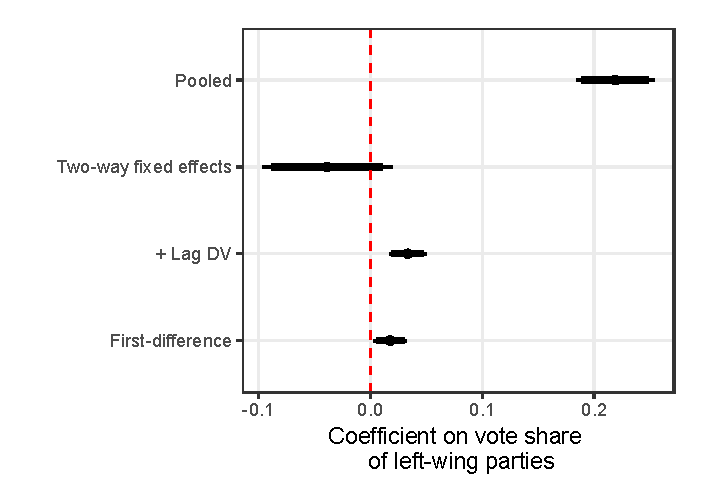
\includegraphics[scale = 1.1]{ggplot_coef_inflation_adjusted.eps}
	\caption{\textbf{Effect of Electoral Support for Right-wing Parties with a 4-year Lead.}} \fnote{\emph{Note: Point are unstandardized OLS coefficients. Lines are 90 pct. (thick) and 95 pct. (thin) confidence intervals computed using Arellano-White robust standard errors clustered at the municipality level, when no lags of the dependent variable are included. Beck-Katz panel-corrected standard errors used for dynamic models. Two and one lags of the dependent variable included, respectively, in the fixed effects and first-difference models.}}
	\label{fig:FourYearLead}
\end{figure}


\begin{figure}[h]
	\centering
	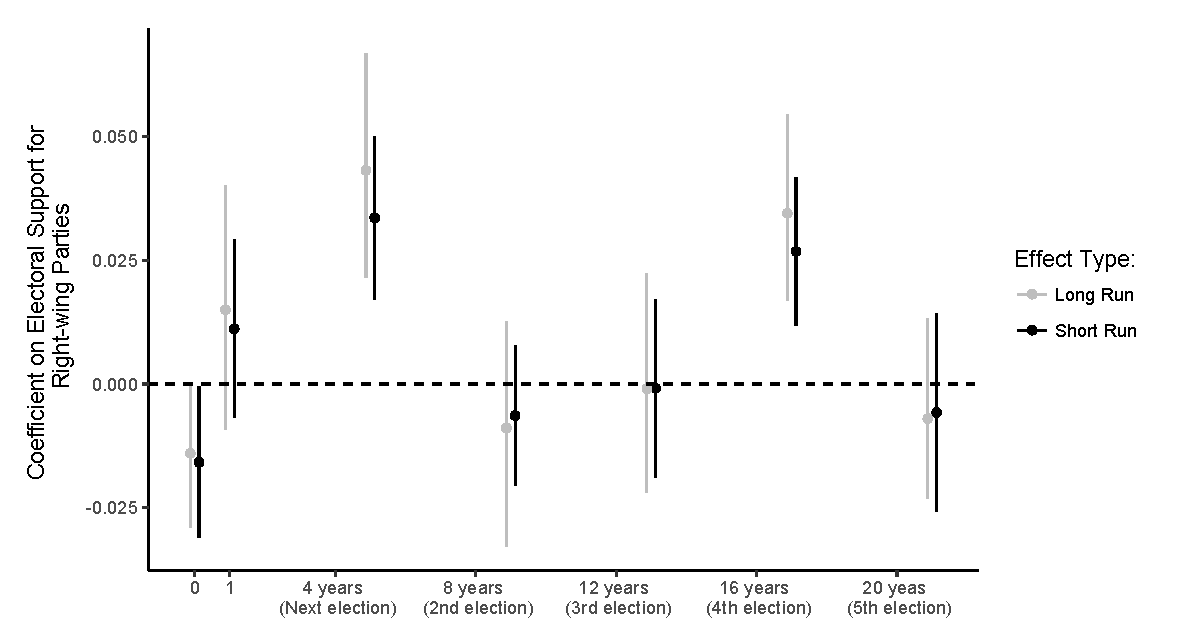
\includegraphics[scale = .8]{coef_on_varying_leads.eps}
	\caption{\textbf{Dynamic Effects of Public Mood.}} \fnote{\emph{Note: Black points represent the effect of electoral support for right-wing parties with different leads. Black lines are 95 pct. confidence intervals based on Arellano-White robust standard errors with municipal clustering. Grey points represent the additional long-run effect of electoral support for right-wing parties due to strong temporal autocorrelation in Fiscal Conservatism. Grey lines are 95 pct. confidence intervals computed from the relevant percentiles of a bootstrapped coefficient distribution based on 1,000 replications and resampling at the municipal level.}}
	\label{fig:LongRun}
\end{figure}



\section{The Effect of Governing Alone: A Discontinuity in Policy Control}

As a final part of our analysis we are interested in examining whether single party majority status affects the level of responsiveness. On the one hand, we might expect single party majority status to hurt responsiveness, since the largest party will then be free to set policy independent of other parties in the city council (parties which also represent parts of the municipal electorate).On the other hand, there might be an accountability effect, where the largest party exerts more effort to align municipal policy with what the electorate prefers if it has a single party majority and thus, in the eyes of the voters, become solely responsible for municipal policy.

We use an RD design to estimate the effect of municipal policy conservatism, comparing the level of responsiveness in municipalities where the largest party narrowly won a majority of the seats in the city council with responsiveness in municipalities where the largest party narrowly lost a majority of the seats. This means focusing on municipal elections where only a few votes were pivotal for giving the largest party a majority of the seats. Below, we describe this design in more detail. This as-if random assignment of single party majority status makes it possible to causally attribute differences in responsiveness to the presence or absence of a single party majority \citep{lee2008randomized,skovron2015practical}.  

\subsection{Identifying close elections}
We identify close elections in a two-step process. In the first step, we single out municipal elections held between 1970 and 2001 where the largest party in the city-council ended up having a one-seat majority or was one seat short of obtaining a majority. This leaves us with 839 close elections out of a pool of 2,475 elections.\footnote{Municipalities with close elections tend to be smaller and more rural than the average municipality, but they resemble the average municipality with respect to the ideological make-up of the electorate and with respect to the tax rate. See section S1 of the supplementary materials for a table that presents these differences.} Figure \ref{figure:closeelec} illustrates this selection process. In the second step, we index the 839 close elections according to \emph{how} close they actually were. That is, we create a forcing variable that can tell us how many additional votes the largest party would have needed to win (lose) in order to have won (lost) the pivotal seat in the city council.


\begin{figure}[htbp] 
	\centering
	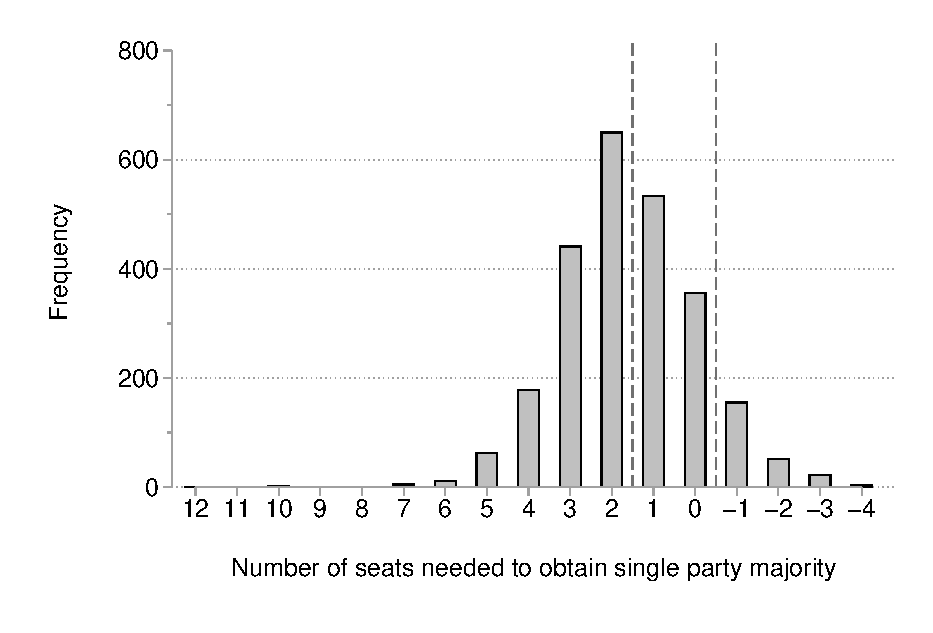
\includegraphics[width=1\textwidth]{closeelec.eps}
	\caption{How many additional seats did the largest party need to obtain a majority? Only elections within the two dashed lines are used in our RD analyses.}
	\label{figure:closeelec}
\end{figure}

Creating the forcing variable, however, is complicated by the fact that there is no joint electoral cut-off at which the largest party is always assigned a majority of the seats in the city council (e.g., 50 pct.). This is not to say that there is no exact cut-off at which majority is assigned in each election; the cut-off simply moves around from election to election. Sometimes it might be 42 pct. and sometimes it might be 45 or 48 pct. 

The varying cut-off is a product of two features of the electoral system in the Danish municipalities. The first feature is that assignment of seats is based on a proportional divisor method. As a consequence, the number seats assigned to the largest party depends on the exact configuration of votes cast for the other parties up for election \citep{fiva2013power,folke2014shades,freier2015parties}. The second feature is that parties can form electoral coalitions \citep{cox1997making}. If parties decide to form an electoral coalition, which they often do, then seats are first assigned to this coalition, and then to the individual parties. As a result, the number of seats assigned to each party depends on the configuration of electoral coalitions, the votes cast for the different electoral coalitions, and the votes cast for the different parties within each coalition.

To develop a forcing variable which takes these particularities of the electoral system into account, we first specified the exact distribution of votes across parties and electoral coalitions for each of the 839 close elections using election reports from Statistics Denmark. Next, we wrote a program that ran simulated elections to determine the number of votes (+/- 10) the largest party would have needed to either win/lose one seat (and thereby secure/lose their majority in the city council).\footnote{In particular, the program added or subtracted 10 votes from the actual vote total of the largest party, while holding the electoral support for the other parties constant, and then calculated the number of seats the largest party would have gotten given the electoral coalitions and the votes cast for other parties. It performed this calculation until the number of seats assigned to the largest party changed, and then reported how many times it had to add or subtract 10 votes before this change had happened. To write this program we used the \texttt{electools} package in Stata \citep{electools}.} Based on this, we measured the number of votes and the proportion of votes that the largest party in the city council would have needed to either win a majority or lose their majority. Figure \ref{figure:forcing} shows how the forcing variable is distributed, that is, exactly how close the 839 close elections were. As can be seen from this figure, there are a large number of elections close to the cut-off (0) in our dataset. In the analyses below, we use the proportional measure as our forcing variable. 



\begin{figure}[htbp] 
	\centering

	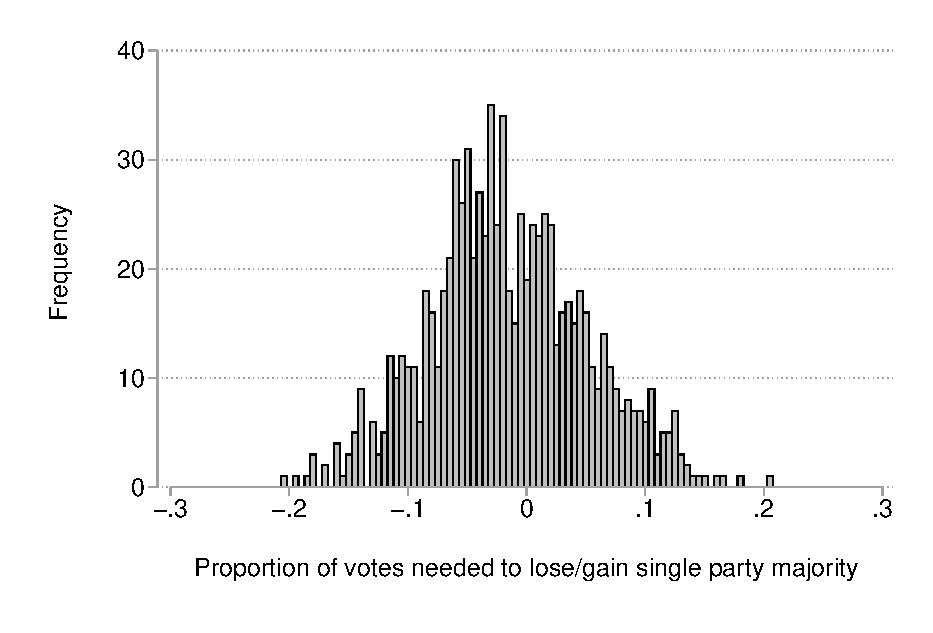
\includegraphics[width=1\textwidth]{distpct.eps}
	\caption{Density of forcing variable measured as proportion of votes. Only calculated for the 839 elections where single party majority status would be reassigned if the largest party either won or lost a single seat.}
	\label{figure:forcing}
\end{figure}

\subsection{A Measure of Responsiveness at the Level of Each Municipality: Congruence}

\subsection{Results}

Figure xx displays our results

\begin{landscape}
	\begin{figure}[h]
		\centering
		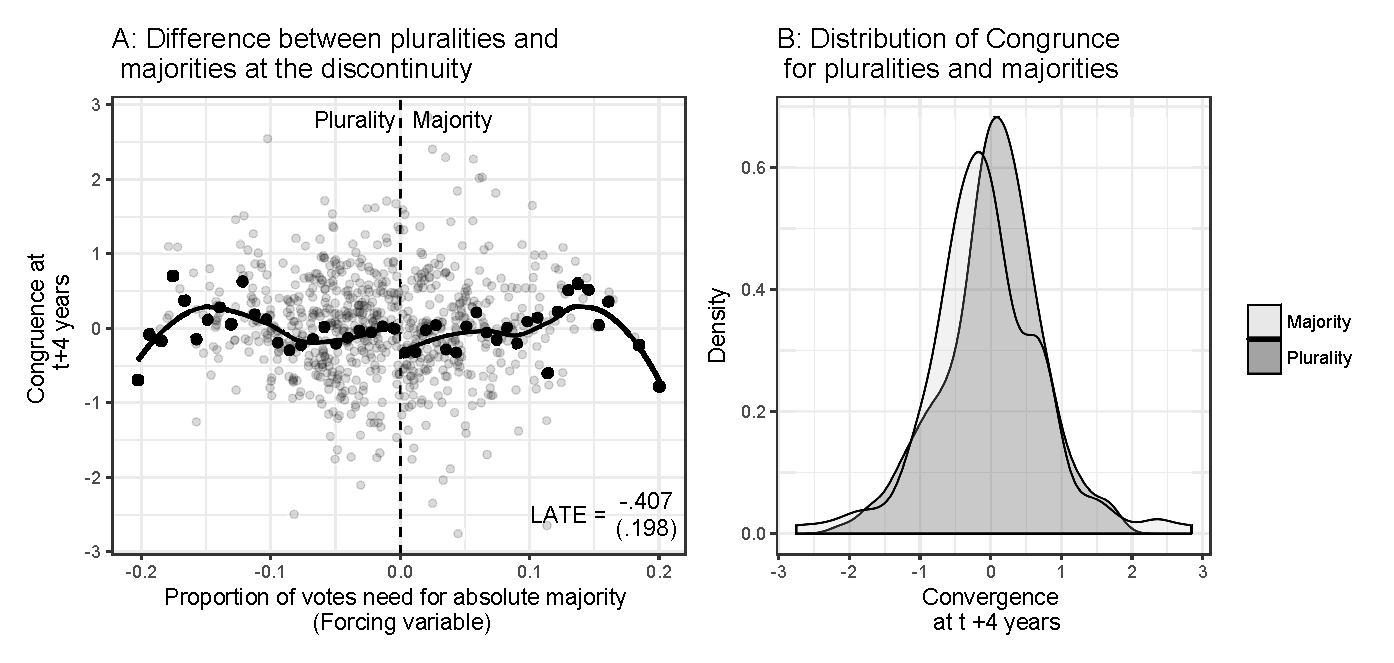
\includegraphics[scale = 1]{rddCongruence.eps}
		\caption{\textbf{.}} \fnote{\emph{Note: .}}
		\label{fig:PermTest}
	\end{figure}
\end{landscape}
	
\section{Conclusion}
This the beginning of a project we hope to extend in various ways. In particular, we currently pondering some of the following questions.
\begin{enumerate}
	\item Are we missing some important policy items? Is it possible to get better coverage for some of the variables? Is it necessary?
	\item  What controls should we have? They need to have good coverage (span all municipalities across many years).
	\item Should we look at a second country? We might be able to do a scaled down version of this in Norway. 
	\item Should we get a better measure of local policy preferences? We think that we will be able to get municipal level ideological estimates by using MRP to model the left-right question in the Danish National Election Studies.
	\item Should we look more into the general responsiveness analysis or more into the RDD? What is the most interesting?
\end{enumerate}

\bibliographystyle{apa}
\bibliography{bibtex/library}


%\beginsupplement

%\section{Supplementary materials}

%\subsection{S1. Descriptive Statistics}

	
\end{document}
